
\documentclass{article}
\usepackage[utf8]{inputenc}     % for éô
\usepackage[danish]{babel}     % for proper word breaking at line ends
\usepackage[a4paper, left=1.5in, right=1.5in, top=1.5in, bottom=1.5in]{geometry}
                                % for page size and margin settings
\usepackage{graphicx}           % for ?
\usepackage{amsmath,amssymb}    % for better equations
\usepackage{amsthm}             % for better theorem styles
\usepackage{mathtools}          % for greek math symbol formatting
\usepackage{enumitem}           % for control of 'enumerate' numbering
\usepackage{listings}           % for control of 'itemize' spacing
\usepackage{todonotes}          % for clear TODO notes
\usepackage{hyperref}           % page numbers and '\ref's become clickable
\usepackage{subcaption}
\usepackage{xcolor}
%\usepackage{allrunes}

%%%%%%%%%%%%%%%%%%%%%%%%%%%%%%%%
%%          TITLE             %%
%%%%%%%%%%%%%%%%%%%%%%%%%%%%%%%%
%             ||               %
%             ||               %
%             \/               %

\def\thesistitle{FinKont0: Fra Itô-calculus til Black-Scholes}
\def\thesissubtitle{Om prisfastsættelse af optioner}
\def\thesisauthorfirst{Jonas}
\def\thesisauthorsecond{Wolff}
\def\thesissupervisorfirst{Prof. Rolf}
\def\thesissupervisorsecond{Poulsen}
\def\thesissecondreaderfirst{Prof. Anders}
\def\thesissecondreadersecond{And}
\def\thesisdate{Juni 2022}


%             /\               %
%             ||               %
%             ||               %
%%%%%%%%%%%%%%%%%%%%%%%%%%%%%%%%
%%          TITLE              %%
%%%%%%%%%%%%%%%%%%%%%%%%%%%%%%%%


%% FOR PDF METADATA
\title{\thesistitle}
\author{\thesisauthorfirst\space\thesisauthorsecond}
\date{\thesisdate}

%% TODO PACKAGE
\newcommand{\towrite}[1]{\todo[inline,color=yellow!10]{TO WRITE: #1}}

%% THEOREM THEMAER
\newtheorem{theorem}{Theorem}[section]
\newtheorem{corollary}{Corollary}[theorem]
\newtheorem{lemma}[theorem]{Lemma}
\newtheorem{proposition}[theorem]{Proposition}

\theoremstyle{definition}
\newtheorem{definition}[theorem]{Definition}

\theoremstyle{remark}
\newtheorem*{remark}{Remark}


%% Dejlige functioner
\DeclareMathOperator{\supersine}{supersin}
\DeclareMathOperator{\supercosine}{supercos}

\newcommand\ens{\Leftrightarrow}
%%%%%%%%%%%%%%%%%%%%%%%

\begin{document}
\begin{titlepage}
	\thispagestyle{empty}
	\newcommand{\HRule}{\rule{\linewidth}{0.5mm}}
	\center
	\textsc{\Large Københavns Universitet}\\[.7cm]
	
\includegraphics[width=25mm]{img/ku_segl.png}\\[.5cm]
	\textsc{Matematisk Institut}\\[0.5cm]
	
	\HRule \\[0.4cm]
	{ \huge \bfseries \thesistitle}\\[0.1cm]
	\textsc{\thesissubtitle}\\
	\HRule \\[.5cm]
	\textsc{\large Bachelor-Projekt i Matematik-Økonomi}\\[.5cm]
	
	\begin{minipage}{0.4\textwidth}
	\begin{flushleft} \large
	\emph{Studerende:}\\
	\thesisauthorfirst\space \textsc{\thesisauthorsecond}
	\end{flushleft}
	\end{minipage}
	~
	\begin{minipage}{0.4\textwidth}
	\begin{flushright} \large
	\emph{Vejleder:} \\
	\thesissupervisorfirst\space \textsc{\thesissupervisorsecond} \\[1em]
	\emph{Censor:} \\
	\thesissecondreaderfirst\space \textsc{\thesissecondreadersecond}
	\end{flushright}
	\end{minipage}\\[4cm]
	\vfill
	{\large \thesisdate}\\
	\clearpage
\end{titlepage}

\tableofcontents

\newpage
\section{Empirisk analyse af lineær SDE}
\subsection{Gaussisk Ornstein-Uhlenbeck proces}
Vi starter med den stochastiske differential ligning nedenfor, hvor efter vi definere processen $Z_t$ og funktionen $f$.

$$\text d X_t = \kappa(\theta - X_t)\text dt+\sigma \text dW_t$$
$$Z_t=e^{\kappa t}X_t,\quad f(x,t)= e^{\kappa t}x$$
Hvor $X_t$ er en process, $W_t$ er en wiener process, og $\kappa,\theta$ og $\sigma$ er konstanter. Vi kan nu bruge Itôs formel
$$\text dZ_t = \kappa e^{\kappa t}X_t\text dt + e^{\kappa t}\text dX_t +\frac12\cdot0\cdot(\text dX_t)^2$$
$$=\kappa e^{\kappa t}X_t\text dt + e^{\kappa t}[\kappa(\theta - X_t)\text dt +\sigma \text dW_t]$$
$$=[\kappa e^{\kappa t}X_t+\kappa e^{\kappa t}(\theta - X_t)]\text dt + e^{\kappa t}\sigma \text dW_t$$
$$=\theta\kappa e^{\kappa t}\text dt + e^{\kappa t}\sigma \text dW_t$$
Nu integrere vi fra t til t+u
$$e^{\kappa(t+u)}X_{t+u}-e^{\kappa t}X_t=\left[\theta e^{\kappa t}\right]_{t}^{t+u}+\int_{t}^{t+u}\sigma e^{\kappa t}\text d W_t$$
$$\ens X_{t+u}=e^{-\kappa u}X_t + e^{-\kappa(t+u)}\left[\theta e^{\kappa t}\right]_{t}^{t+u}+e^{-\kappa(t+u)}\int_{t}^{t+u}\sigma e^{\kappa t}\text d W_t$$
$$=e^{-\kappa u}X_t + \theta(1-e^{-\kappa u})+e^{-\kappa(t+u)}\int_{t}^{t+u}\sigma e^{\kappa t}\text d W_t$$
Her indser vi at det eneste stokastiske i udtrykket er det stokastiske intergrale af en deterministisk funktion med hensyn til en wiener process, selv hvis det er betinget på filtreringen $\mathcal F_t$ som er informationen genereret af $X$ over tidsintervallet $[0,t]$; Dvs, på samme måde som Björk definere det i definition 4.3. Derfor ved vi at $X_{t+u}$ er normalfordelt. Så vi finder nu den betinget middelværdi og varians. Det bruges nedenfor at forventningen til $\text dW_t$ er 0, så det stokastiske intergrale går ud.

$$\text E\left[X_{t+u}|\mathcal F_t\right] = e^{-\kappa u}X_t + \theta(1-e^{-\kappa u}) + e^{-\kappa(t+u)}\text E\left[\int_{t}^{t+u}\sigma e^{\kappa t}\text d W_t|\mathcal F_t\right]$$
$$=e^{-\kappa u}X_t + \theta(1-e^{-\kappa u})$$
$$\text V\left[X_{t+u}|\mathcal F_t\right]= \text E\left[\left(e^{-\kappa(t+u)}\int_{t}^{t+u}\sigma e^{\kappa t}\text d W_t\right)^2|\mathcal F_t\right]$$
$$= e^{-2\kappa(t+u)}E\left[\left(\int_{t}^{t+u}\sigma e^{\kappa t}\text d W_t\right)^2|\mathcal F_t\right]= e^{-2\kappa(t+u)}\text E \left[\int_{t}^{t+u}\sigma^2 e^{2\kappa t}\text (d W_t)^2|\mathcal F_t\right]$$
$$=e^{-2\kappa(t+u)}\text E \left[\int_{t}^{t+u}\sigma^2 e^{2\kappa t}\text dt|\mathcal F_t\right]=e^{-2\kappa(t+u)}\text E \left[\left[\frac{\sigma^2 e^{2\kappa t}}{2\kappa}\right]_{t}^{t+u}|\mathcal F_t\right]$$
$$=e^{-2\kappa(t+u)}\frac{\sigma^2 (e^{2\kappa (t+u)}-e^{2\kappa t})}{2\kappa}=\frac{\sigma^2 (1-e^{-2\kappa u})}{2\kappa}$$
Det vil sige $X_{t+u}|\mathcal F_t\sim\mathcal N\left(e^{-\kappa u}X_t + \theta(1-e^{-\kappa u}),\frac{\sigma^2 (1-e^{-2\kappa u})}{2\kappa}\right)$

\subsection{MLE}
Vi vil nu finde MLE for $\kappa, \theta$ og $\sigma^2$. Dette gøres ved først at lave om parematriseringen 
$$ e^{-\kappa\Delta t}\rightsquigarrow a, \quad \theta(1-e^{-\kappa\Delta t})\rightsquigarrow b, \quad \sigma^2(1-e^{-2\kappa\Delta t})/(2\kappa) \rightsquigarrow v$$
Dvs.
$$\ell(\text{data};a,b,v)=\ln(L(\text{data};a,b,v))=\sum_{i=1}^n \ln\left(\frac1{\sqrt{v2\pi}}e^{-\frac{(x_i-x_{i-1}a-b)^2}{2v}}\right)$$
$$=\sum_{i=1}^n-\frac12\ln(v2\pi)-\frac{(x_i-x_{i-1}a-b)^2}{2v}$$
Vi finder først MLE for $a,b$ og $v$. Nedenfor definere jeg en notation hvor subskriften står får hvor maget bagud lag der er på variablen, f.eks. $x_{01}^s:=\sum_{i=1}^nx_ix_{i-1}$

$$0=\frac{\partial \ell}{\partial a}=\sum_{i=1}^n\frac{x_i-x_{i-1}a-b}{v}x_{i-1}\ens0=\sum_{i=1}^n x_ix_{i-1}-x_{i-1}^2a-bx_{i-1}$$
$$:=x^s_{01}-x^s_{11}a-x^s_1b\ens \hat a=\frac{x_{01}^s-x^s_1\hat b}{x^s_{11}}$$

$$0=\frac{\partial \ell}{\partial b}=\frac{x^s_0-x_1^sa-nb}{v}\ens nb = x_0^s-x_1^s\left[ \frac{x_{01}^s}{x_{11}^s}-\frac{x_1^s}{x_{11}^s}b \right]$$
$$\ens b\left(n-x_1^s\frac{x_1^s}{x_{11}^s}\right)=x_0^s-x_1^s\frac{x_{01}^s}{x_{11}^s}\ens \hat b = \frac{x_0^s-x_1^s\frac{x_{01}^s}{x_{11}^s}}{n-x_1^s\frac{x_1^s}{x_{11}^s}}$$

$$0=\frac{\partial \ell}{\partial v}=\sum_{i=1}^n -\frac12\frac{2\pi}{v2\pi}+\frac{(x_i-x_{i-1}a-b)^2}{2v^2}\ens 0=\sum_{i=1}^n -v+(x_i-x_{i-1}a-b)^2$$
$$\hat v = \frac1n\sum_{i=1}^n(x_i-x_{i-1}\hat a-\hat b)^2$$
Her bør man lægge mærke til at observationerne er antaget ækvidistante så ledes at $\Delta t_i$ kan beskrives med en enkelt konstant $\Delta t$. Dvs., at udledningen ovenfor kun gælder vis obervationerne er ækvidistante. 
MLE for $\kappa,\theta,\sigma^2$ findes ved at sige.
$$e^{-\kappa\Delta t}=\hat a\ens \hat \kappa=\frac{\ln(\hat a)}{-\Delta t}$$
$$\theta(1-e^{-\hat \kappa \Delta t})=\hat b\ens \hat \theta =\frac{\hat b}{1-e^{-\hat \kappa\Delta t}}$$
$$\sigma^2(1-e^{-2\hat\kappa\Delta t})/(2\hat\kappa)=\hat v \ens \hat{\sigma^2}=\frac{2\hat\kappa\hat v}{1-e^{-2\hat\kappa\Delta t}}$$
Vi er dog også intresseret i  konfidensintervallerne for vore parametre, og til det bruger et simulations eksperiment omkring vores MLE'er. Det kunne dog godt tænkes at et smarter trick angående fisher informationen og den asymptotiske statistik lære kunne bruges, men dette er ikke videre undersøgt her.

\subsection{Reality check}
Ved simulation finder vi at MLE'erne passer ret godt. Det gør vi ved at at simulere en process n dage ud i fremtiden som starter i $X_t=100$  hvort efter MLE findes for denne process. Det gentages n\_simul antal gange, og et 95\% konfidensinterval for MLE'erne findes (dvs. der i effekt bare findes 2.5\% og 97.5\% kvantiler) 
\begin{center}
%\begin{table}[]
\begin{tabular}{llllllll}
 &Parametre&& &&& MLE  \\
 $\kappa$&$\theta$&$\sigma^2$&n&n\_simul&$\hat \kappa$&$\hat\theta$&$\hat{\sigma^2}$ \\
 0.1 & 0.1 & 0.1 & 5& 100 & (-0.34, 3.74)&(-1.31, 1.49)&(0.01, 0.56)\\
 0.1 & 0.1 & 0.1 & 100& 100 & (0.06, 0.30)&(-0.52, 0.66)&(0.08, 0.13)\\
 0.05&0.2&0.4&5&100&(-0.25, 2.85)&(-4.79, 9.28)&(0.02, 1.31)\\
 0.05&0.2&0.4&100&100&(0.03, 0.26)&(-1.96, 3.05)&(0.30, 0.49)\\
 0.05&0.2&0.4&1000&100&(0.04, 0.08)&(-0.44, 0.94)&(0.37, 0.44)\\
 0.05&0.2&0.4&10000&100&(0.04, 0.06)&(-0.04, 0.43)&(0.39, 0.41)
\end{tabular}
%\end{table}
\end{center}
Det blev her brugt at observationerne var fordelt med 
$$X_{t+u}|\mathcal F_t\sim\mathcal N\left(e^{-\kappa u}X_t + \theta(1-e^{-\kappa u}),\frac{\sigma^2 (1-e^{-2\kappa u})}{2\kappa}\right)$$ hvor $X_t=100$. Vi ser at at konfidens intervallerne ligger rigtig pænt rundt om de sande parametre. Det virker derfor til at MLE'erne er rigtige. Vi ser også at det kræver ommkring 1000 observationer for at får nogen lunde konfidensintervaller, $\theta$ lader dog til at kræve flere observationer end vi har tester her (Komputer har ikke uandet mængder processor kraft). 
\subsection{log likelihood afledte}
I det næste afsnit får vi brug for vore loglikelihoods afledte. Til det lad os først definere en notation hvor at $f(z_1,\hdots,z_n)_{z_{I_1},\hdots,z_{I_m}}:=\frac{\partial^m f}{\partial z_{I_1}\hdots\partial z_{I_m}}$ hvor $I\in \mathcal P(\mathbb N)$ Dermed får vi resulatterne.
$$\frac{\partial \ell}{\partial \theta}=\sum_{i=1}^n\frac{1}{\phi}\phi_\mu\mu_\theta$$
$$\frac{\partial \ell}{\partial \kappa}=\sum_{i=1}^n\frac1{\phi}(\phi_\mu\mu_\kappa+\phi_{s^2}{s^2}_\kappa)$$
$$\frac{\partial \ell}{\partial \sigma}=\sum_{i=1}^n\frac1{\phi}\phi_{s^2}{s^2}_\sigma$$
$$\mu_\theta = 1-e^{-\kappa\Delta t},\quad \mu_\kappa = x_{i-1}\frac{1}{-\Delta t}e^{-\kappa\Delta t}+\theta\frac{1}{\Delta t}e^{-\kappa\Delta t}$$
$${s^2}_k= \frac{\sigma^2\frac{1}{\Delta t}e^{-2\kappa\Delta t}\kappa-2\sigma^2(1-e^{-2\kappa\Delta t})}{4\kappa^2},\quad {s^2}_\sigma=\sigma\frac{1-e^{-2\kappa\Delta t}}{\kappa}$$
$$\phi_\mu=\frac{y-\mu}{s^3\sqrt{2\pi}}e^{-\frac{(y-\mu)^2}{2s^2}},\phi_{s^2}=-\frac{1}{2(s^22\pi)^{3/2}}2\pi e^{-\frac{(y-\mu)^2}{2s^2}}+\frac{1}{s\sqrt{2\pi}}e^{-\frac{(y-\mu)^2}{2s^2}}\frac{(y-\mu)^2}{2(s^2)^2}$$
De anden afledte lader vi udregne ved numerisk approximation.


%$$\frac{\partial^2 \ell}{\partial \theta^2}=\sum_{i=1}^n-\frac{1}{\phi(i)^2}\phi_\theta\phi_\mu\mu_\theta+\frac1{\phi(i)}\phi_{\mu\theta}\mu_\theta+\frac{1}{\phi(i)}\phi_\mu\mu_{\theta\theta}$$
%$$=\sum_{i=1}^n-\frac{1}{\phi(i)^2}\phi_\theta\phi_\mu\mu_\theta+\frac1{\phi(i)}\phi_{\mu\mu}\mu_\theta\mu_\theta+\frac{1}{\phi(i)}\phi_\mu\mu_{\theta\theta}$$
%$$\frac{\partial^2 \ell}{\partial \theta\partial \kappa}=\sum_{i=1}^n-\frac{1}{\phi(i)^2}\phi_\kappa\phi_\mu\mu_\theta+\frac1{\phi(i)}\phi_{\mu\kappa}\mu_\theta+\frac{1}{\phi(i)}\phi_\mu\mu_{\theta\kappa}$$
%$$\frac{\partial^2 \ell}{\partial \theta\partial \sigma}=\sum_{i=1}^n-\frac{1}{\phi(i)^2}\phi_\sigma\phi_\mu\mu_\theta+\frac1{\phi(i)}\phi_{\mu\sigma}\mu_\theta+\frac{1}{\phi(i)}\phi_\mu\mu_{\theta\sigma}$$
\subsection{Det asymptotiske konfidensinterval}
Det er et velkendt resultat at normal fordeling er en eksponentiel familie, og vi kan der medbruge lauritzen 2021's Theorem 4.11 til at sige.
$$(\hat\kappa,\hat\theta,\hat{\sigma^2})\overset{as}{\sim}\mathcal N_3((\kappa,\theta,\sigma^2),\tilde{i}_n (\kappa,\theta,\sigma^2)^{-1})$$
Det vil sige at har vi fisher informationen $\tilde{i}_n (\kappa,\theta,\sigma^2)^{-1})$ så lan vi finde $1-\alpha$ konfidenstinervallet som.
$$(\hat\kappa,\hat\theta,\hat{\sigma^2})\pm \sqrt{tr(\tilde{i}_n (\hat\kappa,\hat\theta,\hat{\sigma^2})^{-1})}\gamma_{1-\alpha/2}$$
Hvor $\gamma_{1-\alpha/2}$ er standard normalfordelingens $1-\alpha/2$ kvantilen, og $\tilde i_n$ er defineret som
$$\tilde{i}_n (\zeta):= -\text E\left[D^2\ell (\zeta,X_1,\hdots,X_n)\right]$$
Med $\zeta := (\kappa,\theta,\sigma^2)$. Man kunne nu ønske sig at sammenligne dette konfidensinterval med det simuleret konfidensinterval, omend bare for at validere vores asymptotiske konfidensinterval mod det mere simple simuleret konfidensinterval, som man som læser nok har mere tidlig til er udført rigtigt.
\begin{center}
%\begin{table}[]
\begin{tabular}{llllllll}
 &Parametre&& &&& MLE  \\
 $\kappa$&$\theta$&$\sigma^2$&n&n\_simul&$\hat \kappa$&$\hat\theta$&$\hat{\sigma^2}$ \\
 0.1 & 0.1 & 0.1 & 5& 100 & (-0.65, 1.56)&(-1.57, 0.39)&(-0.08, 0.28)\\
 0.1 & 0.1 & 0.1 & 100& 100 & (0.07, 0.08)&(-0.06, 0.53)&(0.08, 0.10)\\
 0.05&0.2&0.4&5&100&(-0.54, 1.47)&(-3.24, 0.94)&(-0.52, 2.4)\\
 0.05&0.2&0.4&100&100&(0.12, 0.15)&(0.85, 1.89)&(0.42, 0.55)\\
 0.05&0.2&0.4&1000&100&(0.070, 0.073)&(0.05, 0.47)&(0.39, 0.42)\\
 0.05&0.2&0.4&10000&100&(0.0486, 0.0494)&(-0.02, 0.13)&(0.400, 0.405)
\end{tabular}
%\end{table}
\end{center}
Ud fra dette kan man konludere at de asymptotiske konfidens intervaller ser ud til at være mindre end vores simuleret konfidens intervaller. Metoden hvor på disse asymptotiske konfidens intervaller er udregnet på er dog ved at approksimere den anden afledte. Man kunne tro at dette ikke var en helt præcis approximation som dermed kunne give forkerte resultater. 
\subsection{VIX}
Vi prøver nu at bruge teorien på Yahoo Finance's VIX data. Dette giver os MLE'erne.
$$\hat \kappa=0.024 ,\quad \hat \theta =20.27,\quad \hat{\sigma^2}= 4.27$$
Vi prøver nu at finde konfidens intervallerne for $\hat\kappa,\hat \theta$, og $\hat{\sigma^2}$, som gøres ved at bruge MLE'erne som de sande parametre, og da bruge samme simmulations trick, som i forrige afsnit til at finde konfidensintervallerne. n er her lig antal observatione, dvs. 3800, og n\_simul er sat til at vøre 100.
 $$\hat\kappa\in(0.0171443652522532,0.0310665609921349)$$
 $$\hat\theta\in(17.5496619191198 ,23.3745635491285)$$
 $$\hat{\sigma^2}\in(4.10458482202505,4.45763390757801)$$
Vi prøver nu at finde konfidens intervallerne for $\hat\kappa,\hat \theta$ og $\hat{\sigma^2}$ under antagelsen at logaitmen til VIX følger en lineær SDE.
$$\hat \kappa=0.021 ,\quad \hat \theta =2.93,\quad \hat{\sigma^2}= 0.0062$$
 $$\hat\kappa\in(0.0171703975760097,0.0278142219595335)$$
 $$\hat\theta\in(2.81171168885257 ,3.00801217792473)$$
 $$\hat{\sigma^2}\in(0.00597746278029887,0.00647443568140169)$$
Hvilket virker som et meget sensibelt resultat. Vi kan nu bruge vores MLE til at plotte en simulation af vores process, samt VIX-dataen, med og uden logaritme antagelsen for at se hvilken der passer bedst.
\begin{figure}
\centering
\begin{subfigure}{2in}
    \raggedright
    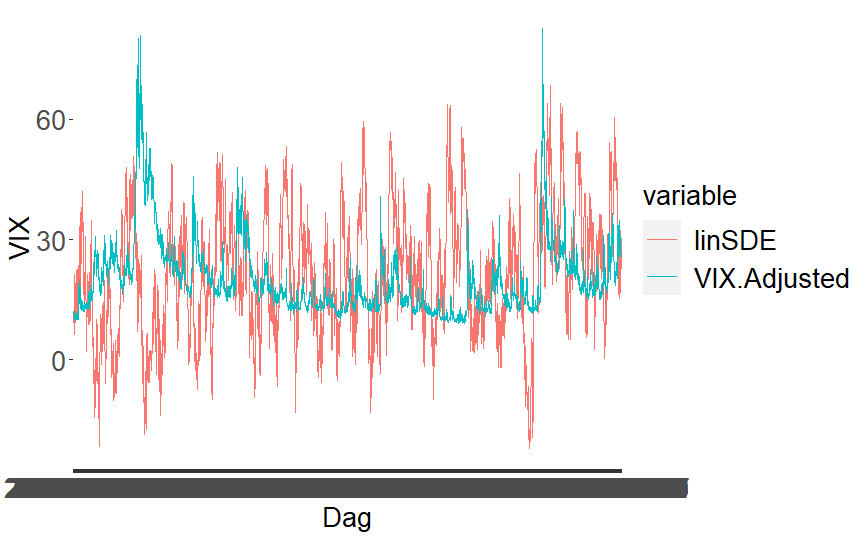
\includegraphics[width=2in]{Rplot27}
    \caption{VIX vs. SDE}
    \label{fig:VIX}
\end{subfigure}
\begin{subfigure}{2in}
    \raggedleft
    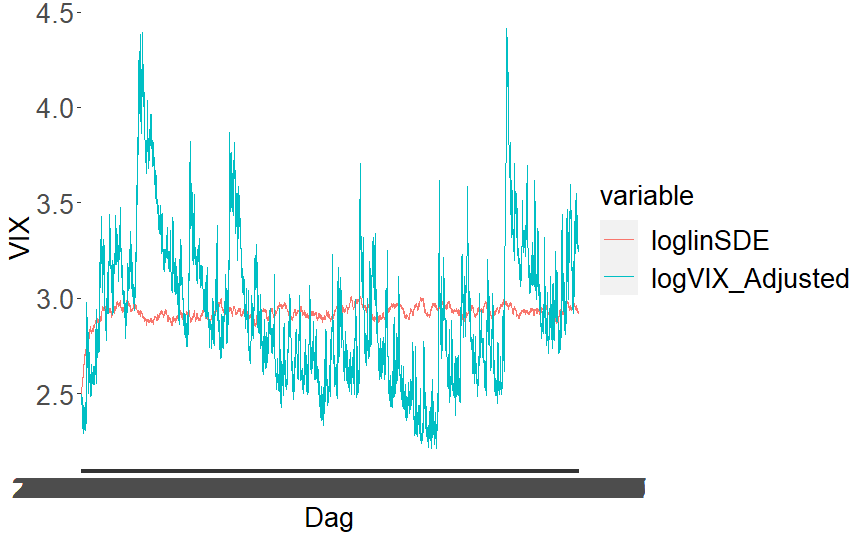
\includegraphics[width=2in]{Rplot28}
    \caption{lnVIX vs. SDE}
    \label{fig:logVIX}
\end{subfigure}
\end{figure}
man ser her at vores process følger ln(VIX) bedre en med VIX. Vi kan også kigge på vores antagelse om at VIX er normalfordelt. Nedenfor ses 2 QQ-plot
\begin{center}
    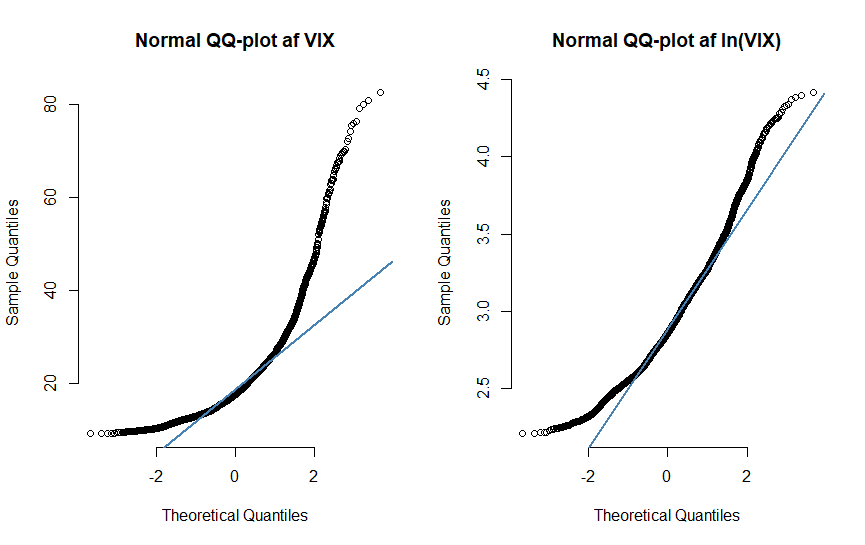
\includegraphics[width=4in]{Rplot17.png}
\end{center}
Her ses det at ln(VIX) ligger mere normal fordelt i forhold til kvantilerne end VIX gør. Vi kan derfor konkludere at ln(VIX)-modellen passer bedst til dataen
\section{Pricing and hedging in the Black-Scholes model}
\subsection{Europæisk call option}
Til at starte med udledes et brugbart resultat. Vi definere først en stokastisk differential ligning.
$$\text d X_t = \beta X_t\text dt+\xi X_t \text dW_t$$
Og funktionen samt procesen.
$$f(t,x)=e^{(\beta-\alpha)(T-t)}x,\quad Y_t=f(t,X_t)=e^{(\beta-\alpha)(T-t)}X_t$$
Vi kan nu finde $X_t$ ved brug af itô's formel.
$$\text dY_t=-(\beta-\alpha)e^{(\beta-\alpha)(T-t)}X_t\text d_t+e^{(\beta-\alpha)(T-t)}\text dX_t$$
$$=-(\beta-\alpha)e^{(\beta-\alpha)(T-t)}X_t\text dt+e^{(\beta-\alpha)(T-t)}(\beta X_t\text dt+\xi X_t\text dW_t)$$
$$=e^{(\beta-\alpha)(T-t)}X_t(\beta-(\beta-\alpha))\text dt+\xi X_t\text dW_t$$
$$=-e^{(\beta-\alpha)(T-t)}X_t\alpha\text dt+\xi X_t\text dW_t$$
Vi bruger Björks proposition 7.13, hvor ligning (7.53) og (7.54) giver os at
$$d_1(t,Y_0) :=\frac{1}{\xi\sqrt{T-0}}\left[\ln\left(\frac{Y_0}{K}\right)+(\alpha+\frac12\xi)(T-0) \right]$$
$$=\frac{T(\beta-\alpha)+\ln\left(\frac{X_0}{K}\right)+(\alpha+\frac12\xi)T}{\xi\sqrt T}=\frac{\ln\left(\frac{X_0}{K}\right)+(\beta+\frac12\xi^2)T}{\xi\sqrt T}$$
$$d_2(t,Y_0):=\frac{\ln\left(\frac{X_0}{K}\right)+(\beta+\frac12\xi^2)T}{\xi\sqrt T}-\xi\sqrt{T}$$
$$=\frac{\ln\left(\frac{X_0}{K}\right)+(\beta+\frac12\xi^2)T-\xi^2T}{\xi\sqrt T}=\frac{\ln\left(\frac{X_0}{K}\right)+(\beta-\frac12\xi^2)T}{\xi\sqrt T}$$
Og dermed får vi det nyttige resultat.
$$F(t,Y_0)=Y_0\Phi(d_1)-e^{-\alpha T}K\Phi(d_2)$$
$$=e^{(\beta-\alpha)T}X_0\Phi\left(\frac{\ln\left(\frac{X_0}{K}\right)+(\beta+\frac12\xi^2)T}{\xi\sqrt T}\right)-e^{-\alpha T}K\Phi\left(\frac{\ln\left(\frac{X_0}{K}\right)+(\beta-\frac12\xi^2)T}{\xi\sqrt T}\right)$$
Endvidere kunne vi tænke os at finde tid $t-\Delta$'et for en call-option i markedet.
$$\text dB_t = rB_t\text d_t$$
$$\text d S_t = \mu S_t\text d_t +\sigma \text dW_t^P$$
P skal her forstås som aktie-pris dynamikken. Pris processen $B_t$ er her det risiko fri aktiv, og pris-processen $S_t$ for aktie kuren. $\mu,\sigma$ og $r$ er konstanter. Björks proposition 7.13 fortæller os nu at tid-t prisen på den europæiske call option er.
$$\Pi_t=F(t,S_t)=S_t\Phi\left(\frac{\ln\left(\frac{S_t}{K}\right)+(r+\frac12\sigma^2)(T-t)}{\sigma\sqrt{T-t}}\right)-e^{-r(T-t)}\Phi\left(\frac{\ln\left(\frac{S_t}{K}\right)+(r-\frac12\sigma^2)(T-t)}{\sigma\sqrt{T-t}}\right)$$
$$:= S_t\Phi(d_1^a)-e^{-r(T-t)}\Phi(d_2^a)$$
tid t-$\Delta$'et er da
$$\Delta(S_t,t) = \frac{\partial \Pi_t}{\partial S_t}=\Phi(d_1^a)+S_t\frac{\phi(d_1^a)}{S_t\sigma\sqrt{T-t}}-e^{-r(T-t)}K\frac{\phi(d_2^a)}{S_t\sqrt{T-t}}$$
$$=\Phi(d_1^a)+\frac{X_t\phi(d_1^a)-e^{-r(T-t)}K\phi(d_2^a)}{S_t\sigma\sqrt{T-t}}=\Phi(d_1^a)+\frac{S_t\phi(d_1^a)-S_t\phi(d_1^a)}{S_t\sigma\sqrt{T-t}}=\Phi(d_1^a)$$
Her er det brugt at $\phi(d_2^a)=\phi(d_1^a)\frac{S_t}{K}e^{r(T-t)}$, og at standard normalfordelingens tætheds funktion er navngivet $\phi$. Neden for vises udledning af vores trick.
$$\phi(d_2^a)=\phi(d_1^a-\sigma\sqrt{T-t})=\frac{1}{\sqrt{2\pi}}e^{-\frac12\left[(d_1^a)^2+\sigma^2(T-t)-2d_1^a\sqrt{T-t}\right]}$$
$$=\phi(d_1^a)e^{-\frac12\left[\sigma^2(T-t)-2d_1^a\sqrt{T-t}\right]}=\phi(d_1^a)e^{-\frac12\left[\sigma^2(T-t)-2\frac{\ln\left(\frac{S_t}{K}\right)+(r+\frac12\sigma^2)(T-t)}{\sigma\sqrt{T-t}}\sqrt{T-t}\right]}=\phi(d_1^a)\frac{S_t}{K}e^{r(T-t)}$$
\subsection{Digital option}
Lige ledes vil vi nu finde prisen på en digital option. Til det bruges Björks ligning (7.50), Q står her for det risiko neutrale mål. Vi definere også et $\\Z\sim\mathcal N((r-\frac12\sigma^2)(T-t),\sigma\sqrt{T-t})$ og ligeledes dens henholdvise tæthedsfunktion $\phi_Z$ og fordelingsfunktion $\Phi_Z$. 
$$E^Q_{t,S_t}\left[1_{S_T\leq K}\right]=\int_{-\infty}^{\infty}1_{S_te^{z}\leq K}\phi_Z(z)\text dz=\int_{-\infty}^{\ln\left(\frac K{S_t}\right)}\phi_Z(z)\text d z=\Phi_Z\left(\ln\left(\frac{K}{S_t}\right)\right)$$
$$\ens \Pi_t=F(t,S_t)=e^{-r(T-t)}\Phi_Z\left(\ln\left(\frac{K}{S_t}\right)\right)$$
Vi er ligeledes intresseret i den tid-t $\Delta$, som findes nedenfor.
$$\Delta(S_t,t)=\frac{\partial \Pi_t}{\partial S_t}=e^{-r(T-t)}\phi_Z\left(\ln\left(\frac{K}{S_t}\right)\right)\frac{1}{K/S_t}\left(-\frac{K}{S_t^2}\right)=-e^{-r(T-t)}\phi_Z\left(\ln\left(\frac{K}{S_t}\right)\right)\frac{1}{S_t}$$

\subsection{Hedging af en europæisk call option}
Et R program skrevet af Rolf Poulsen der hedger optioner kan findes \href{https://www.dropbox.com/s/ykq11phsrk2ho89/DiscreteBlackScholesDeltaHegdeOfCall.R?dl=0}{Her}. Koden udregner blandt andet for en europæisk call option antal aktier i det underliggende aktiv og værdi investeret i bankbogen ved brug af Bkörks Theorem 8.5 til at replikere call optionen, som blandt andet siger at.
$$h^S_t=\frac{\partial \Pi_t}{\partial S_t}$$
$$h^B_tB_t=\Pi_t-S_t\frac{\partial \Pi_t}{\partial S_t}$$
Hvor $h^S_t$ skal forstås som antal aktier i det underliggende aktiv $S_t$, og $h^B_t$ som antal aktier i det risikofri aktiv (Dvs. $h^B_tB_t$ er antal kr. i bankbogen). Ud fra det kan den replikerende porteføljes værdi udregnes som
$$V^h_t=h^s_tS_t+h^B_tB_t=\Pi_t$$
Disse værdier udregnes Nhedge antal gange inden for løbetiden, med ækvidistante mellem rum. Man kan nu gøre dette et hvis antal gange (her kaldet Nrep) sammenligne den replikerende porteføljes værdi, og optionens værdi $V^{Call}_t=\max(S_t-K,0)$ f.eks. som gjordt i koden ved at tage gennemsnitet af de tilbage diskonteret værdier. 

Skulle man være i en situation, hvor det underliggende aktivs drift ikke er lig bankbogens rente, da vil det bryde med antagelsen om at vi kan bruge de risikofri mål $\mathbb Q$ i black-scholes, og dermed skabe størrer afvigelser mellem de endelige porteføljens værdier og optionens værdier. Dette er fordi at hvis man værdi ansætter aktiver med et risikofrit mål, da gives der ikke præmier for påtaget risiko, og alle aktiver burde da have den samme drift. Som det kan ses i figur \ref{fig:my_label4}
\begin{figure}{3in}
    \centering
    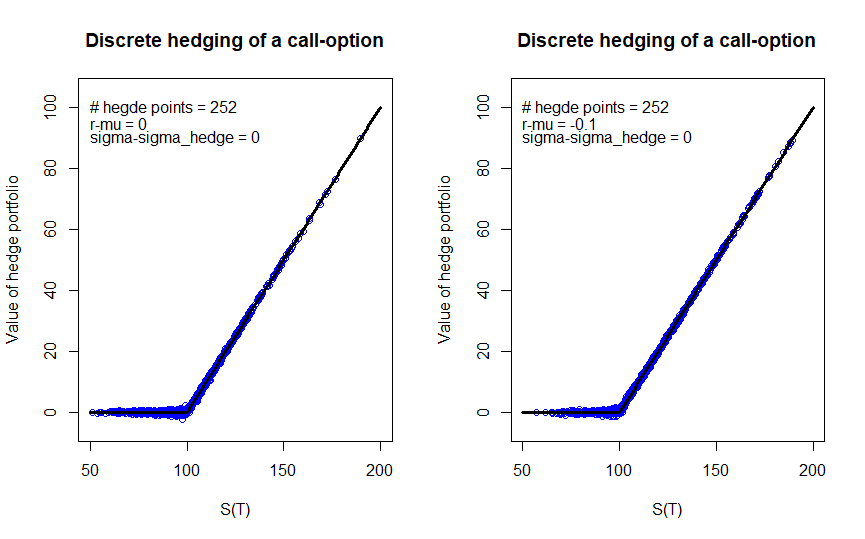
\includegraphics[width=3.5in]{Rplot24.png}
    \caption{Endelig Hedge afvigelse i gns. hhv 0.328992810316579 og 0.309239380268836}
    \label{fig:my_label4}
\end{figure}

I tilfældet af at man ikke har fundet det rigtige $\sigma$ til at bruge i black-scholes, da ser vi også at de andelige afvigelser mellem den replikerende portefølje og optionen øges. Dette er på grund af at teorien antager at vi bruger volatiliteten der faktisk er på det risiko fyldte aktiv. Dette ses i figur \ref{fig:my_label5}
\begin{figure}{3in}
    \centering
    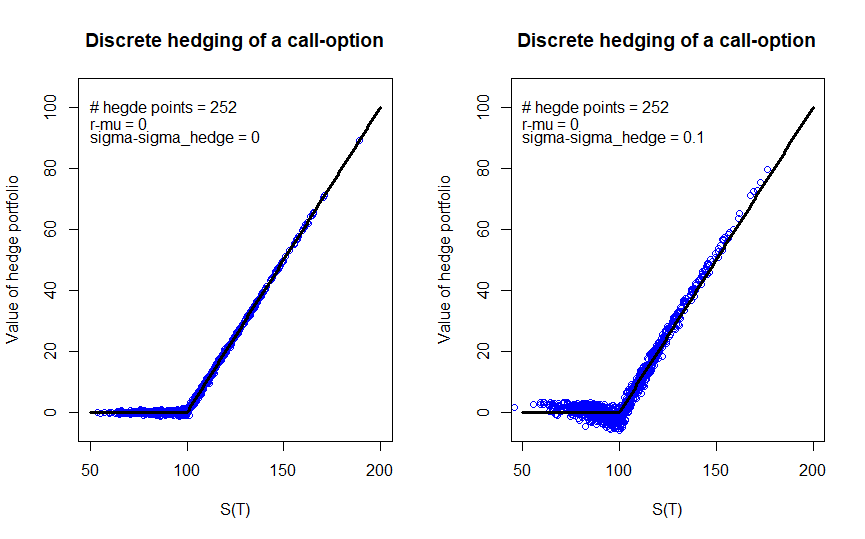
\includegraphics[width=3.5in]{Rplot25.png}
    \caption{Endelig Hedge afvigelse i gns. hhv 0.318458605758955 og 1.69360232996912}
    \label{fig:my_label5}
\end{figure}

I forhold til at føre Björks Theorem 8.5 ud i livet har vi også et problem i forhold til at modellen antager at vi rebalancere kontinuert over løbetiden, hvilket som bekendt er umuligt. Derfor må vi approksimere os ved at rebalancere så ofter som muligt; Det betyder også at jo flere gange ve rebalancere, jo mere præcis bliver vores delta hedging. Standard afvigelsen på forskellen mellem den replikerende portefølje og option stiger derfor jo færre rebalanceringer vi laver (Det der i koden kaldes Nhedge). Det tilhørende resultat fides i figur \ref{fig:my_label6}.
\begin{figure}{3in}
    \centering
    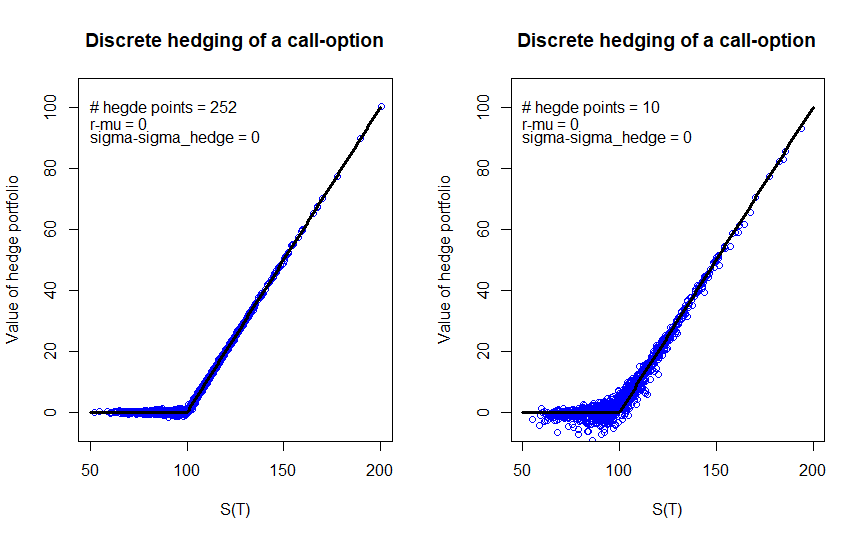
\includegraphics[width=3.5in]{Rplot26.png}
    \caption{Endelig Hedge afvigelses sd. hhv 0.429390437548319 og 2.16104852090886}
    \label{fig:my_label6}
\end{figure}

Kigger vi derimod på den digitale option, ser vi at præcisionen ikke afhænger notitsværdigt af om driften er lig renten, selvom vi stadig gøre brug af Q-målet. På den anden side bliver vi meget afhængige af om vores estimeret sigma\_hedge faktisk er det rigtige sigma, da et forkert sigma\_hedge vil øge forskellen mellem den den replikerende portefølje og optionen. Antalet at rebalanceringer Nhedge, her også en ret stpr betydning da vores option payoff ikke er kontinuert, og vi derfor her brug for rebalanceringer ret tæt omkring striken, og da vores rebalncering i vores teori skal være ækvidistante, kan vi ikke gøre andet end at øge antallet af rebalnceringer. Neden for vises simulationerne. Resultatet ses i figure \ref{fig:my_label3}, \ref{fig:my_label2} og \ref{fig:my_label1}.
\begin{figure}{3in}
    \centering
    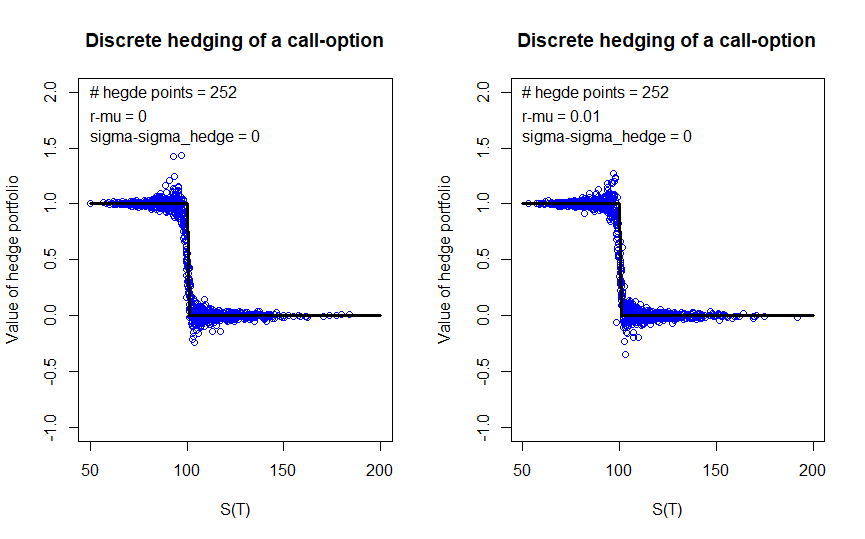
\includegraphics[width=3.5in]{Rplot21.png}
    \caption{Endelig Digital Hedge afvigelse i gns. hhv 0.0460204036853945 og 0.0494517674871319}
    \label{fig:my_label3}
\end{figure}
\begin{figure}{3in}
    \centering
    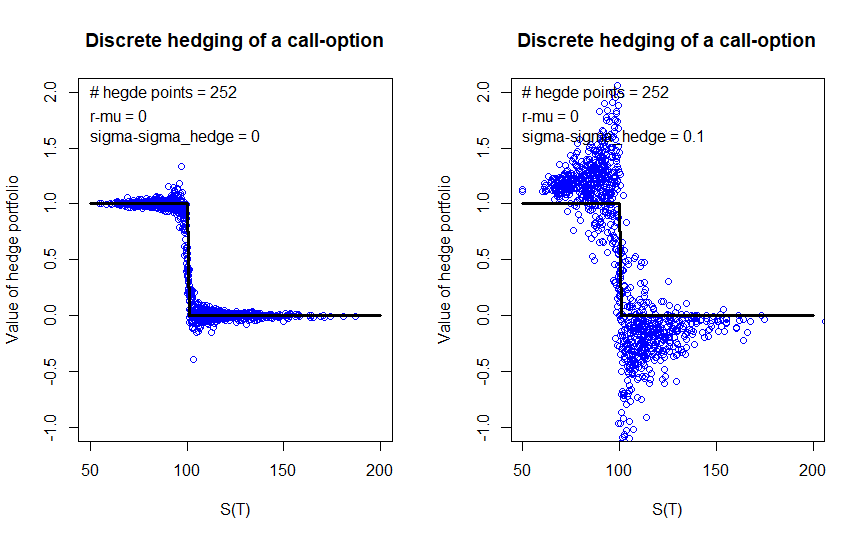
\includegraphics[width=3.5in]{Rplot22.png}
    \caption{Endelig Digital Hedge afvigelse i gns. hhv 0.0460204036853945 og 0.265897800975727}
    \label{fig:my_label2}
\end{figure}
\begin{figure}{3in}
    \centering
    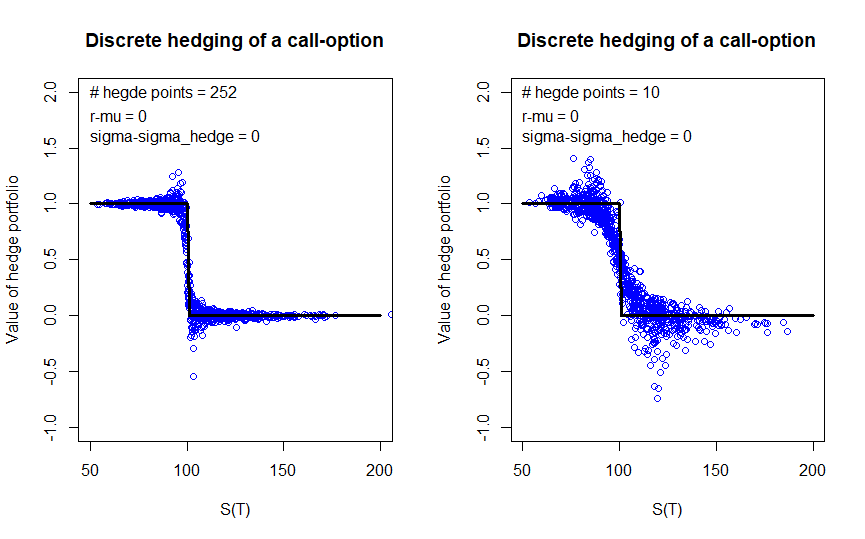
\includegraphics[width=3.5in]{Rplot23.png}
    \caption{Endelig Digital Hedge afvigelses sd. hhv 0.105776252993221 og 0.207893956373506}
    \label{fig:my_label1}
\end{figure}



\subsection{No touch digital option}
Præcis samme argumentation som i den almindelige digital option kan bruges her igen, hvor vi definere $M_t=\max_{0\leq u\leq t}S_u$ som værende payoff for vores no touch digitale option
$$E^Q_{t,M_t}\left[1_{M_T\leq K}\right]=\int_{-\infty}^{\infty}1_{\max_{0\leq u\leq t} (S_ue^{z})\leq K}\phi_Z(z)\text dz=\int_{-\infty}^{\infty}1_{e^{z}M_t\leq K}\phi_Z(z)\text dz$$
$$=\int_{-\infty}^{\ln\left(\frac K{M_t}\right)}\phi_Z(z)\text d z=\Phi_Z\left(\ln\left(\frac{K}{S_t}\right)\right)\ens \Pi_t=F(t,S_t)=e^{-r(T-t)}\Phi_Z\left(\ln\left(\frac{K}{M_t}\right)\right)$$

\section{Empirical hedging}
Vi vil nu udvide vore experiment til S\&P500, som ses på firgur \ref{fig:VIXSP500}, hvor den første dato på både VIX og S\&P500 er normeret til 100, så de kan sammenlignes.
\begin{figure}
    \centering
    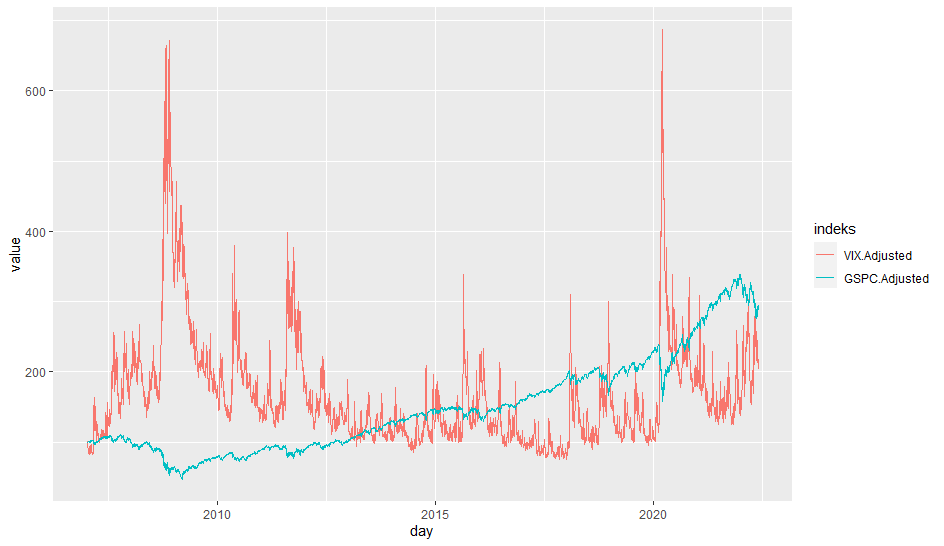
\includegraphics[width=3.5in]{Rplot30.png}
    \caption{En graf over VIX of S\&P500, normeret}
    \label{fig:VIXSP500}
\end{figure}
Her ses det at S\&P500 har langt mindre volatilitet, og vi kan tydeligt se tæt på konstant drift, man kunne derfor tænke sig at sige at denne er tættere på at kunne simuleres af en geometrisk brownsk bevægelse, da eftersom at driften er næsten konstant.



\newpage



\bibliographystyle{plain}
\bibliography{references.bib}

\end{document}

